\section{Ergebnisse der Hyperparameter-Optimierung und des Trainings}
\subsection{Hyperparameter-Optimierung von \MiniDog{}}

In \autoref{fig:hyper-param} ist das Ergebnis der Hyperparameter-Optimierung von \MiniDog{}
dargestellt. Die optimalen Hyperparameter sind eine \texttt{Batch Size} von 2,
eine Stärke von 0.001 der \texttt{L2-Regularisierung} und die Verwendung
der Farbinformationen.

\begin{figure}
  \centering
  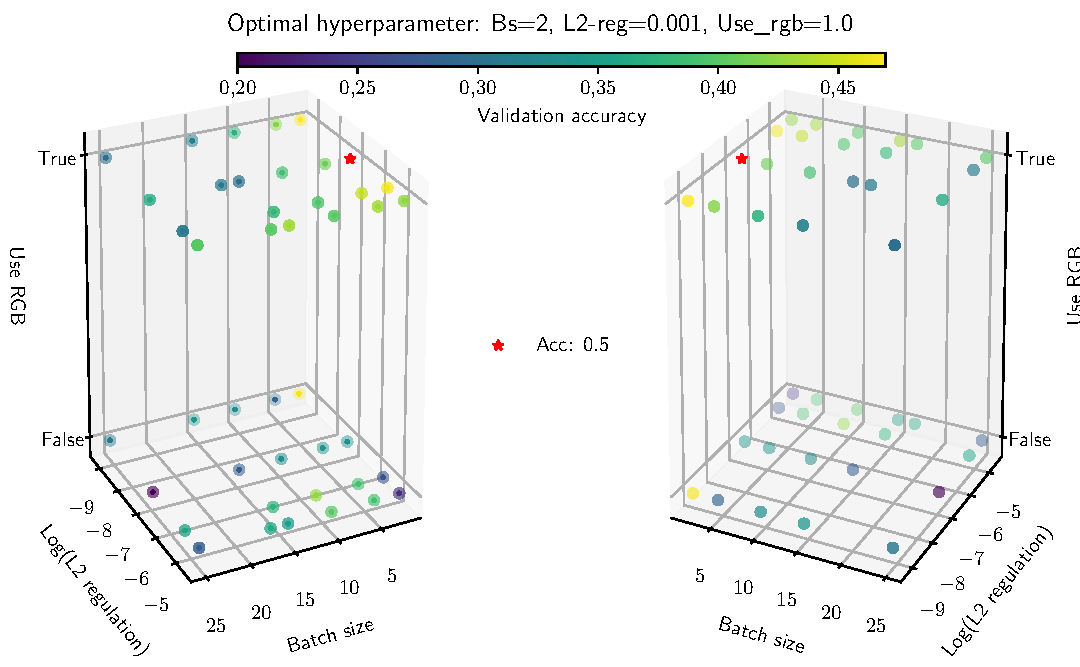
\includegraphics[scale=0.6]{pics/ergebnisse/hyper_raum.pdf}
  \caption{Darstellung der Ergebnisse der Hyperparameter-Optimierung
  von \MiniDog{}. Die beste Kombination ist als Stern dargestellt und wurde auch
  für das Training verwendet.}
  \label{fig:hyper-param}
\end{figure}

Allgemein wird ersichtlich, dass in den meisten Fällen die Verwendung von Farbinformationen
zu einer höheren Validation Accuracy führt. Also kann eine der Fragen, ob die Verwendung
von Farbinformationen einen Vorteil in der Klassifikation bringt, mit Ja beantwortet werden.

\subsection{Verschiedene Bildgrößen beim  Training von \PreDog{} und \PreBig{}}

Wie bereits in \autoref{sec:größe-bilder} beschrieben, wurde für die beiden
Neuronalen Netze, die ein vortrainiertes Netz nutzen, alle Bilder 125x138
geresized. Dies erreichte eine Validation Accuracy von ungefähr \SI{60}{\percent}.
Falls die Bilder aber auf 224x224 geresized werden, dann steigt die Accuracy
auf ungefähr \SI{95}{\percent}. Da im kleinen Datensatz nur maximal 74 Bilder
kleiner sind als 224x224, die Validation Accuracy aber deutlich besser ist, wird diese Methode zum Training verwendet.
Loss und Accuracy Kurven sind im Anhang zu finden.

\subsection{\PreBig{}}

\begin{wrapfigure}{r}{11.2cm}
  \centering
  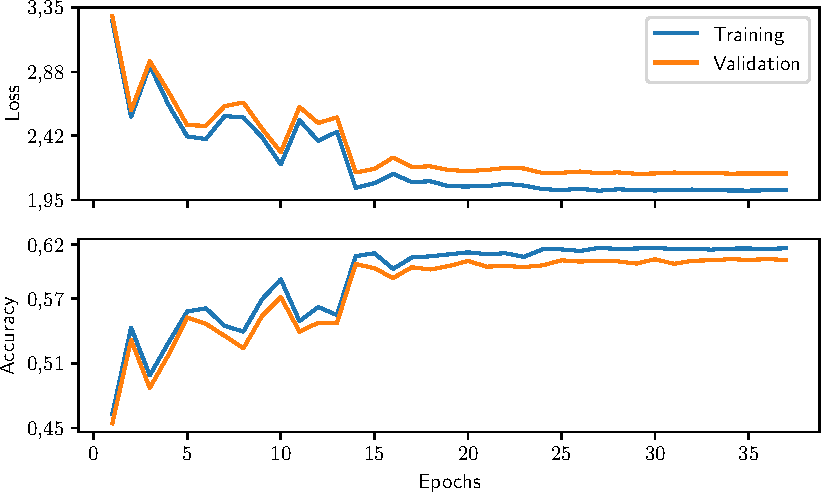
\includegraphics[scale=0.8]{pics/ergebnisse/PreBigDogNN/history_epoch.pdf}
  \caption{Loss und Accuracy Kurven für \PreBig{}.}
  \label{fig:loss-acc-prebig}
\end{wrapfigure}

In \autoref{fig:loss-acc-prebig} sind die Loss und Accuracy Kurven für \PreBig{}
zu sehen. Ungefähr ab Epoche 14 ist leichtes Overtraining zu erkennen. Hier
wäre eine Anpassung der \texttt{dropout-rate} und der Stärke der \texttt{L2-Regularisierung}
Mögliche Stellschrauben, um das Overtraining zu beseitigen, möglicherweise im Zuge
einer umfassenden Hyperparameter-Optimierung.

Die Confusion-Matrix zeigt eine deutliche Diagonale, was als gut zu bewerten ist.
Allerdings werden einzelne Klassen noch häufig falsch klassifiziert, zum Beispiel
ist ein vom Netz als American Staffordshire Terrier klassifizierter Hund zu ungefähr
\SI{80}{\percent} ein Staffordshire Bullterrier. Die Ähnlichkeit der beiden Rassen
steckt schon im Namen und wird bei genauerer Betrachtung der Bilder beider Klassen
deutlich. Alles in allem funktioniert die Klassifikation gut, einzelne Klassen
wie z.\.B. der African Hunting Dog werden (fast) immer richtig klassifiziert.

\begin{figure}
  \centering
  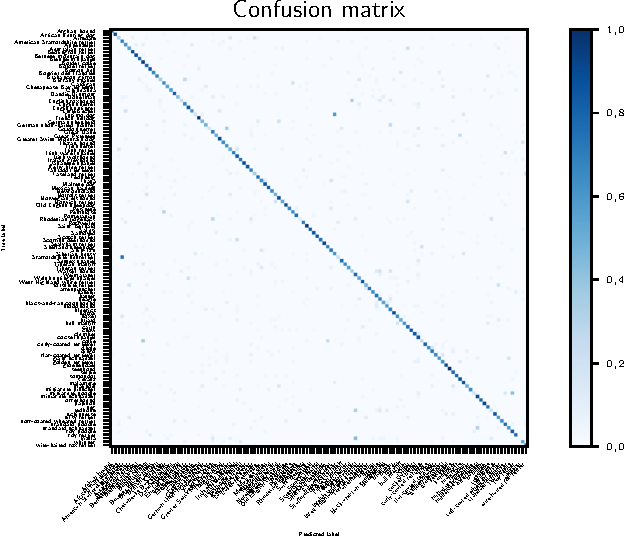
\includegraphics[scale=0.8]{pics/ergebnisse/PreBigDogNN/confusion_matrix.pdf}
  \caption{Confusion Matrix für \PreBig{}.}
  \label{fig:confusion-prebig}
\end{figure}

\subsection{\MiniDog}

\begin{wrapfigure}{r}{11.2cm}
  \centering
  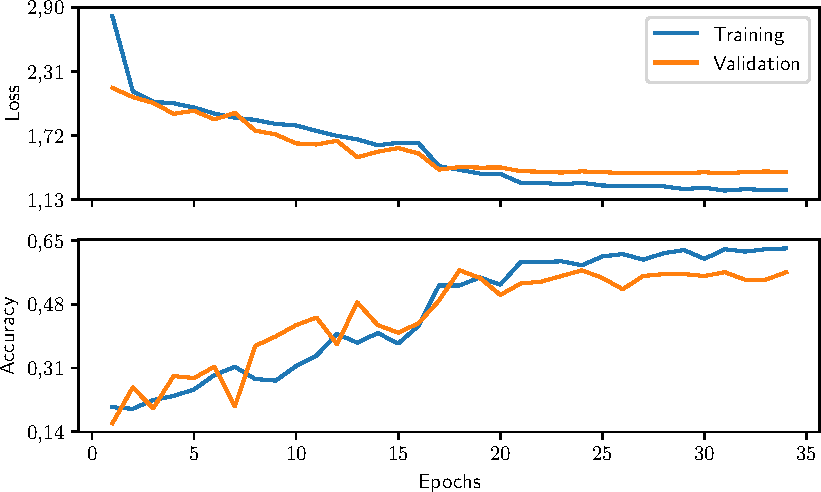
\includegraphics[scale=0.8]{pics/ergebnisse/MiniDogNN/history.pdf}
  \caption{Loss und Accuracy Kurven für \MiniDog{}.}
  \label{fig:loss-acc-minidog}
\end{wrapfigure}

In \autoref{fig:loss-acc-minidog} sind die Loss und Accuracy Kurven für \MiniDog{}
trainiert auf 5 Klassen zu sehen. Auch hier ist ab Periode 25 leichtes
Overtraining zu erkennen, welches mit stärkerer \texttt{L2-Regularisierung} oder
früherem Abbruch beseitigt werden könnte.

\autoref{fig:confusion-mini} zeigt die Confusion-Matrix des Trainings aus
\autoref{fig:loss-acc-minidog}. Es zeigt sich, dass der African Hunting Dog im
Vergleich zu den anderen Klassen sehr gut, am schlechtesten ist der Schipperke
zu klassifizieren. Dies zeigt sich auch in \autoref{fig:visualize-pred}. Dort
wurde der Schipperke am wahrscheinlichsten als African Hunting Dog
klassifiziert, was sich auch in der Confusion-Matrix zeigt. Bis auf den African
Hunting Dog in \autoref{fig:visualize-pred} entsprechen die wahrscheinlichsten
Predictions nicht den True Labeln. Hier ist also noch Verbesserungspotential,
z.\,B. durch eine umfassende Hyperparameter-Optimierung.

In \autoref{fig:confusion-mini-120} ist die Confusion-Matrix von \MiniDog{} für
120 Klassen dargestellt ist. Es wird sofort ersichtlich, dass die Klassifikation
nicht gut funktioniert hat, da alle Bilder einer einzelnen Klasse zugeordnet
werden. Damit wird auch klar, dass nicht mit dem gleichen Netz 5 und 120 Klassen
gut klassifiziert werden können.

\begin{figure}
  \begin{subfigure}{0.49\textwidth}
    \centering
    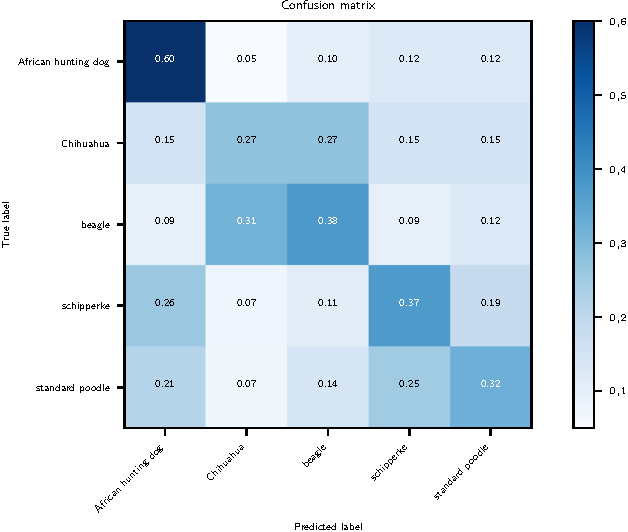
\includegraphics[width=\textwidth]{pics/ergebnisse/MiniDogNN/confusion_matrix}
    \caption{Confusion-Matrix für das Training von \MiniDog{}.}
    \label{fig:confusion-mini}
  \end{subfigure}
  \begin{subfigure}{0.49\textwidth}
    \centering
    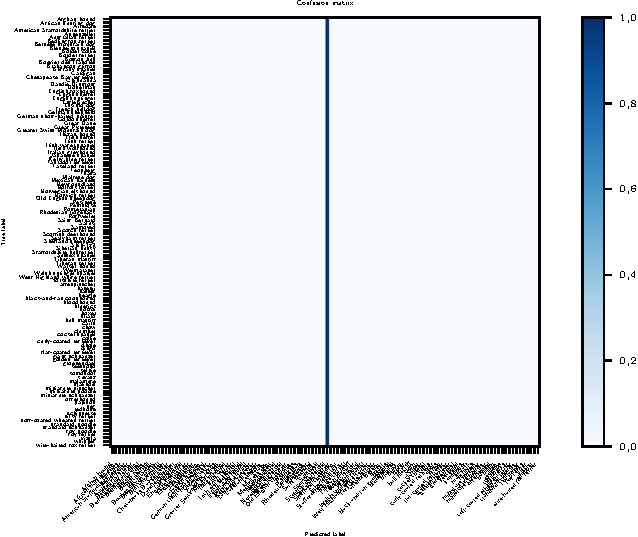
\includegraphics[width=\textwidth]{pics/ergebnisse/MiniDogNN/confusion_matrix_mini120.pdf}
    \caption{Confusion Matrix für \MiniDog{}, trainiert auf 120 Klassen.}
    \label{fig:confusion-mini-120}
  \end{subfigure}
  \caption{Confusion-Matrizen für \MiniDog{} für den kleinen und den großen Datensatz.}
  \label{fig:confusion-mini-gesamt}
\end{figure}

% \begin{figure}
%   \centering
%   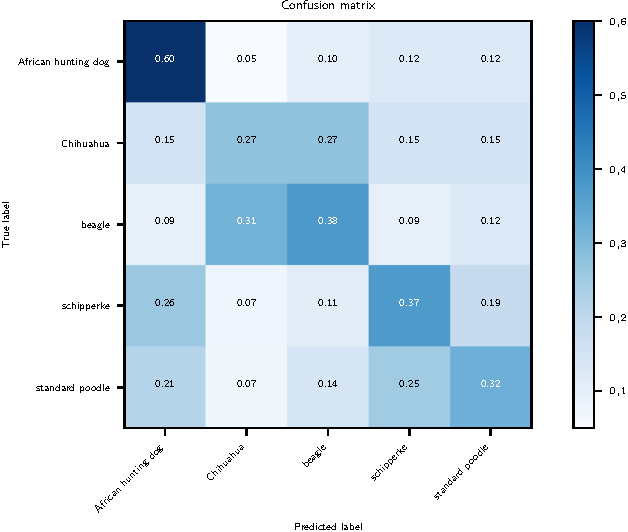
\includegraphics[scale=0.8]{pics/ergebnisse/MiniDogNN/confusion_matrix}
%   \caption{Confusion-Matrix für das Training von MiniDogNN.}
%   \label{fig:confusion-mini}
% \end{figure}

\begin{figure}
  \centering
  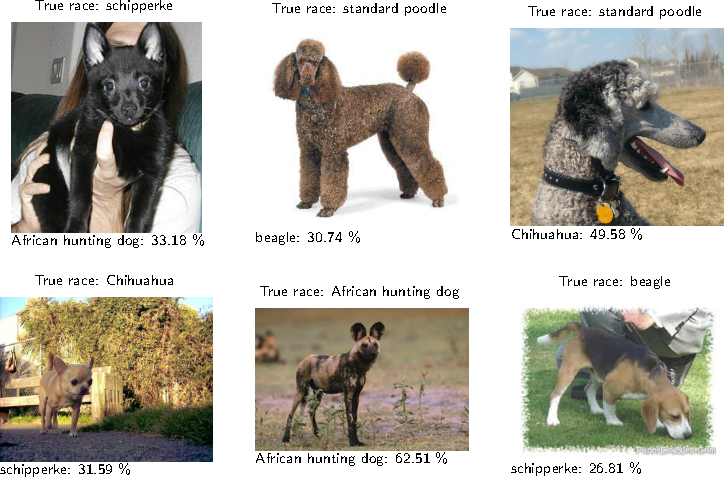
\includegraphics[scale=0.8]{pics/ergebnisse/MiniDogNN/visualize_predictions.pdf}
  \caption{Auswahl von sechs Bilder aus dem Testdatensatz des kleinen
  Datensatzes für \MiniDog{} mit den jeweilig wahrscheinlichsten Predictions.}
  \label{fig:visualize-pred}
\end{figure}

% \begin{figure}
%   \centering
%   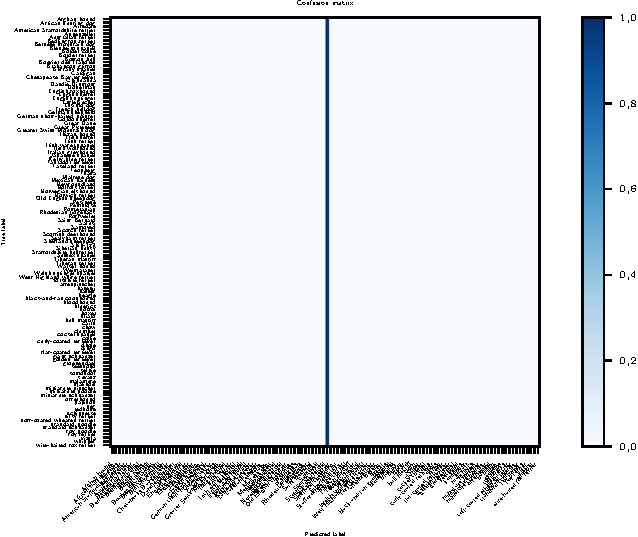
\includegraphics{pics/ergebnisse/MiniDogNN/confusion_matrix_mini120.pdf}
%   \caption{Confusion Matrix für \MiniDog, trainiert auf 120 Klassen.}
%   \label{fig:confusion-mini-120}
% \end{figure}

\subsection{\PreDog}

\begin{figure}
  \centering
  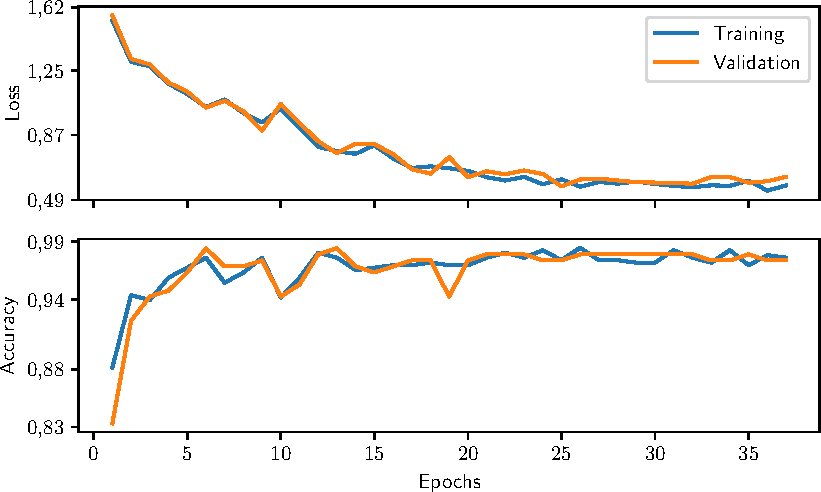
\includegraphics[scale=0.8]{pics/ergebnisse/PreDogNN/history_epoch.pdf}
  \caption{Loss und Accuracy Kurven für \PreDog{}.}
  \label{fig:loss-acc-predog}
\end{figure}

In \autoref{fig:loss-acc-predog} sind die Loss und Accuracy Kurven für \PreDog{} zu sehen.
Es ist kein Overtraining zu erkennen, was als positiv zu bewerten ist.

Die Confusion-Matrix in \autoref{fig:confusion-predog} zeigt, dass das Training sehr gut
verlaufen ist. Beagle, Schipperke und Standard Poodle werden mit \SI{100}{\percent}-tiger
Wahrscheinlichkeit richtig erkannt; bei African Hunting Dog und Beagle werden teilweise
noch falsche Klassifizierungen vorgenommen, allerdings nur \SI{3}{\percent} bzw.
\SI{12}{\percent}. Somit lässt sich sagen, dass unter Verwendung des vortraininerten
Netzes die Klassifikation deutlich besser verläuft als bei \MiniDog{}.

\begin{figure}
  \centering
  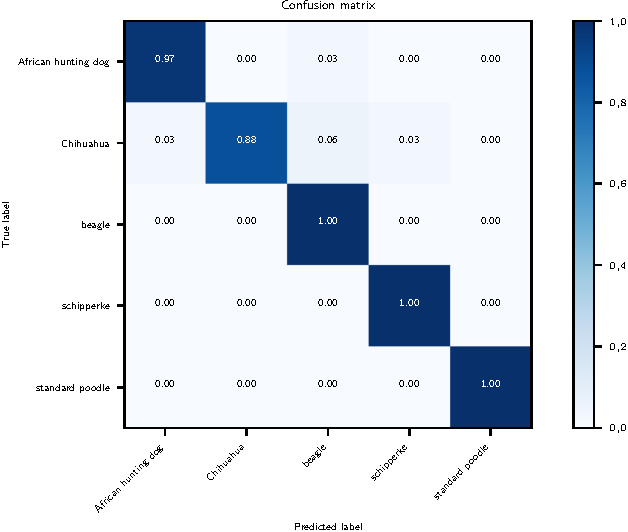
\includegraphics[scale=0.8]{pics/ergebnisse/PreDogNN/confusion_matrix.pdf}
  \caption{Confusion-Matrix für \PreDog{}.}
  \label{fig:confusion-predog}
\end{figure}

\subsection{\RF}

\begin{figure}
  \centering
  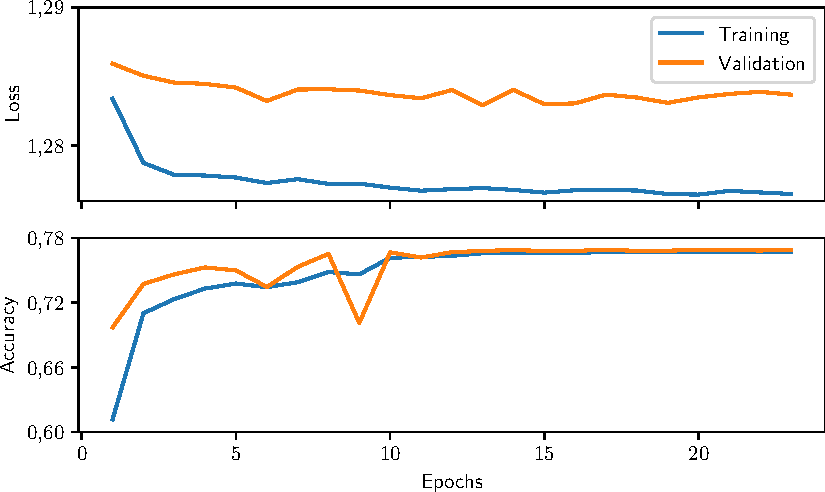
\includegraphics[scale=0.8]{pics/ergebnisse/RF/history.pdf}
  \caption{Loss und Accuracy Kurven für den Autoencoder des Random Forest,
  trainiert auf 120 Klassen.}
  \label{fig:loss-acc-rf}
\end{figure}

In \autoref{fig:loss-acc-rf} sind die Loss und Accuracy Kurven für den Autoencoder
des Random Forest dargestellt. Dabei wurde der Autoencoder auf 120 Klassen trainiert.
Aus der Loss-Kurve wird ersichtlich, dass Overtraining vom Start weg gegeben ist.
Die Accuracy kann das nicht unterstützen. Allerdings ist das Overtraining klein,
weswegen es in der Accuracy wahrscheinlich nicht sichtbar ist.

Die Confusion-Matrizen aus \autoref{fig:confusion-rf} zeigen, dass einerseits
die Klassifizierung in \autoref{sub:confusion-rf-120} besser funktioniert hat
als in \autoref{fig:confusion-mini-120}, aber andererseits schlechter als in
\autoref{fig:confusion-prebig}. Die Confusion-Matrizen für den kleinen Datensatz
sind schwieriger zu vergleichen im Hinblick auf \MiniDog{}, allerdings wird auch
hier ersichtlich, dass die Klassifikation mit einem vortrainierten Netz deutlich
besser funktioniert als in \autoref{fig:confusion-mini} und
\autoref{sub:confusion-rf-5}.

\begin{figure}
  \begin{subfigure}{0.49\textwidth}
    \centering
    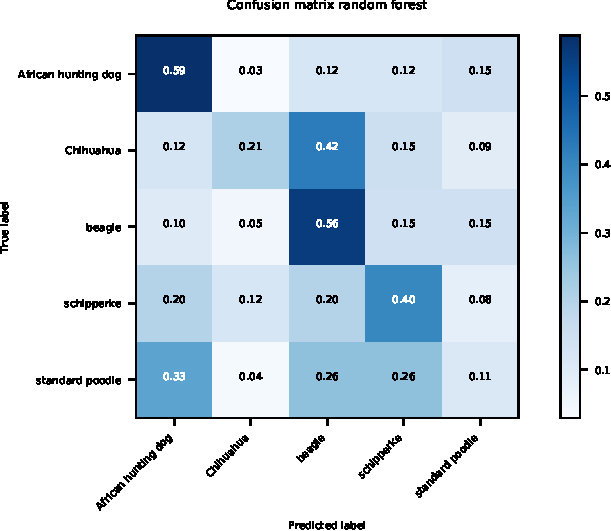
\includegraphics[width=\textwidth]{pics/ergebnisse/RF/confusion_matrix_rf.pdf}
    \caption{Confusion-Matrix für die Klassifizierung des Random Forest auf 5 Klassen.}
    \label{sub:confusion-rf-5}
  \end{subfigure}
  \qquad
  \begin{subfigure}{0.49\textwidth}
    \centering
    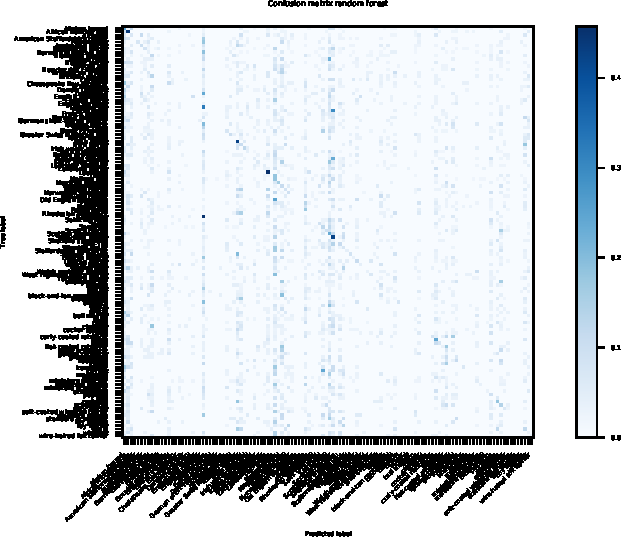
\includegraphics[width=\textwidth]{pics/ergebnisse/RF/confusion_matrix_big.pdf}
    \caption{Confusion-Matrix für die Klassifizierung des Random Forest auf 120 Klassen.}
    \label{sub:confusion-rf-120}
  \end{subfigure}
  \caption{Darstellung der Confusion-Matrizen für 5 und 120 Klassen.}
  \label{fig:confusion-rf}
\end{figure}
